\section{Traction}
\label{sec:traction}

Section~\ref{sec:drivetrain} showed that traction caps how much of the motors' torque the robot can use, so the track surface is the most leveraged part of the drivetrain.

The stock tracks are hard plastic links: they provide almost no friction, and using them, our robot was unable to climb at all. The final surface is strips of 80 grit sandpaper taped onto the stock tracks (Fig.~\ref{fig:tracks}).

\begin{figure}[htbp]
  \centering
  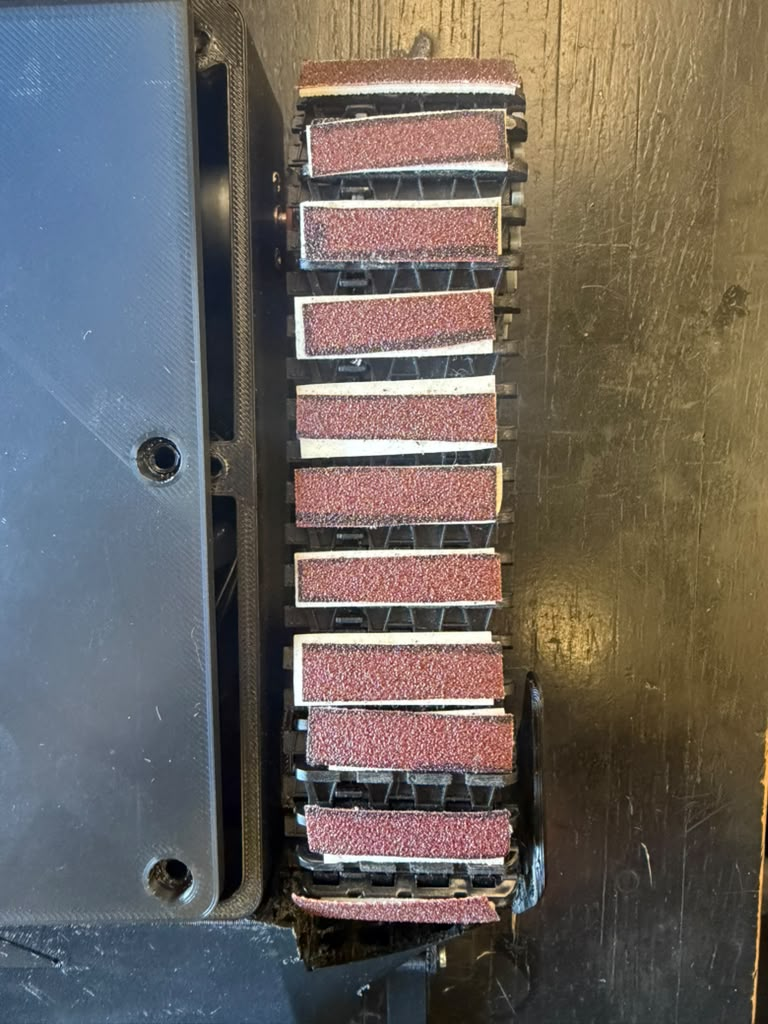
\includegraphics[width=0.34\textwidth]{fig05_tracks.jpg}
  \caption{\tbd{Caption.}}
  \label{fig:tracks}
\end{figure}

% we haven't done this - if we don't ever end up doing this we need a backup plan
To measure $\mu_s$ we \tbd{placed the robot on the ramp surface and raised the angle until it slipped, so \mbox{$\mu_s = \tan\theta_\mathrm{slip}$}; or pulled it with a luggage scale until it slid, so \mbox{$\mu_s = F/N$}}. We tested each surface \tbd{three times at each of three normal forces, adding \_\_\_ g of mass between sets} (Table~\ref{tab:friction}).

\begin{table}[htbp]
  \centering
  \caption{Measured static friction coefficients.}
  \label{tab:friction}
  \begin{tabular}{@{}l c c c c c@{}}
    \toprule
    Surface & Normal force (\unit{N}) & Trial 1 & Trial 2 & Trial 3 & Mean $\mu_s$ \\
    \midrule
    Stock tracks & \tbd{\ } & \tbd{\ } & \tbd{\ } & \tbd{\ } & \tbd{\ } \\
    Stock tracks & \tbd{\ } & \tbd{\ } & \tbd{\ } & \tbd{\ } & \tbd{\ } \\
    Stock tracks & \tbd{\ } & \tbd{\ } & \tbd{\ } & \tbd{\ } & \tbd{\ } \\
    \midrule
    Sandpaper    & \tbd{\ } & \tbd{\ } & \tbd{\ } & \tbd{\ } & \tbd{\ } \\
    Sandpaper    & \tbd{\ } & \tbd{\ } & \tbd{\ } & \tbd{\ } & \tbd{\ } \\
    Sandpaper    & \tbd{\ } & \tbd{\ } & \tbd{\ } & \tbd{\ } & \tbd{\ } \\
    \bottomrule
  \end{tabular}
\end{table}

\tbd{Result: sandpaper raised \mbox{$\mu_s$} from \_\_\_ to \_\_\_, which by Eq.~\eqref{eq:traction} raises the most force the tracks can transmit on the ramp from \_\_\_ to \_\_\_ N.}
